\chapter{Pré-traitement d'image\\ (Adrian \& Thibault)}

La bibliothèque SDL permet facilement de manipuler et charger des images, et
cela pour n'importe quel type de format (PNG, JPEG, BMP, \ldots). Il a donc
fallu dans un premier temps se familiariser avec cette bibliothèque à l'aide de
la documentation en ligne ainsi que du TP 3 de nos cours de programmation en C.

\section{Niveau de gris}

Transformer une image avec un niveau de gris est une opération basique de
traitement d'image. Pour cela, nous appliquons à chaque pixel la formule de la
luminance :

$L = 0.2126 \cdot R + 0.7152 \cdot G + 0.0722 \cdot B$

\begin{figure}[H]
    \centering
    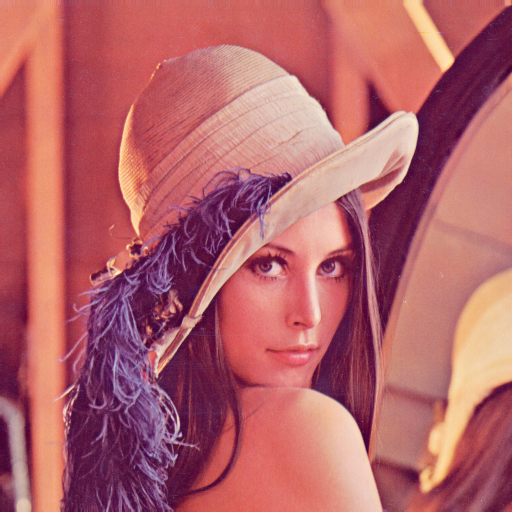
\includegraphics[width=0.3\textwidth]{lenna}
    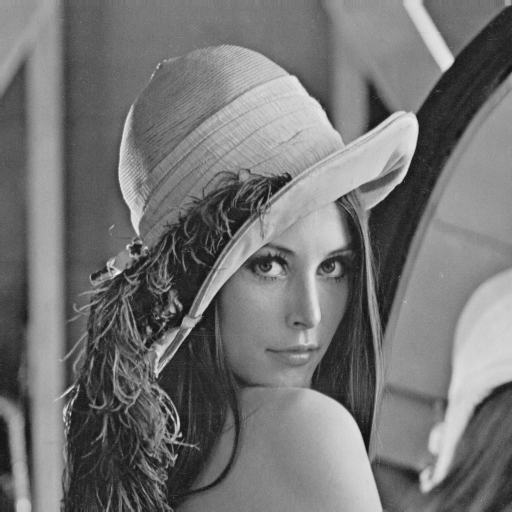
\includegraphics[width=0.3\textwidth]{lenna_gray}
    \caption{Niveau de gris}
\end{figure}

\section{Binarisation}

Pour binariser une image, la première étape est de choisir un seuil. Ce dernier
détermine si un pixel sera blanc ou noir (en fonction de s'il est inférieur ou
supérieur à ce seuil). Plusieurs méthodes existent pour choisir ce seuil, on
peut distinguer deux catégories :

\begin{itemize}
    \item \textbf{seuil fixe} : pour toutes les images un seuil est choisi pour
        décider si un pixel sera blanc ou noir.
    \item \textbf{seuil automatique} : chaque image est analysée pour déterminer
        un seuil adapté à cette dernière.
\end{itemize}

Sélectionner un seuil fixe est une solution facile à mettre en place mais peut
donner des résultats très variés en fonction de la qualité de l'image, de sa
luminosité ou encore des contrastes.

\begin{figure}[H]
    \centering
    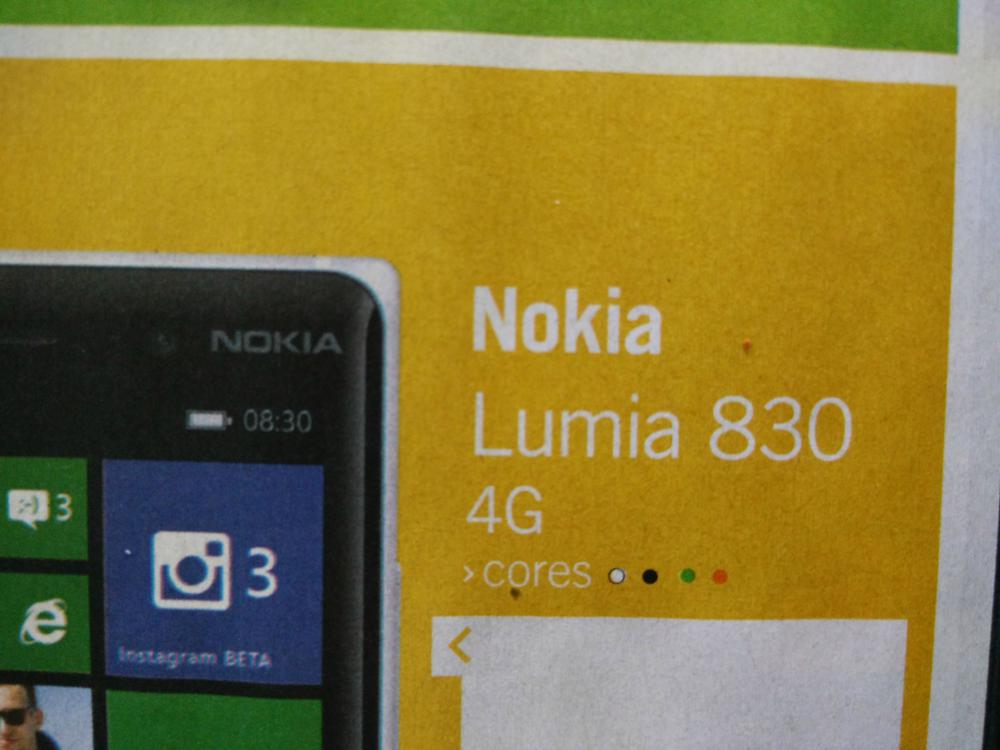
\includegraphics[width=0.4\textwidth]{fixed_threshold_00}
    \caption{Image originale en couleur}
\end{figure}

\begin{figure}[H]
    \centering
    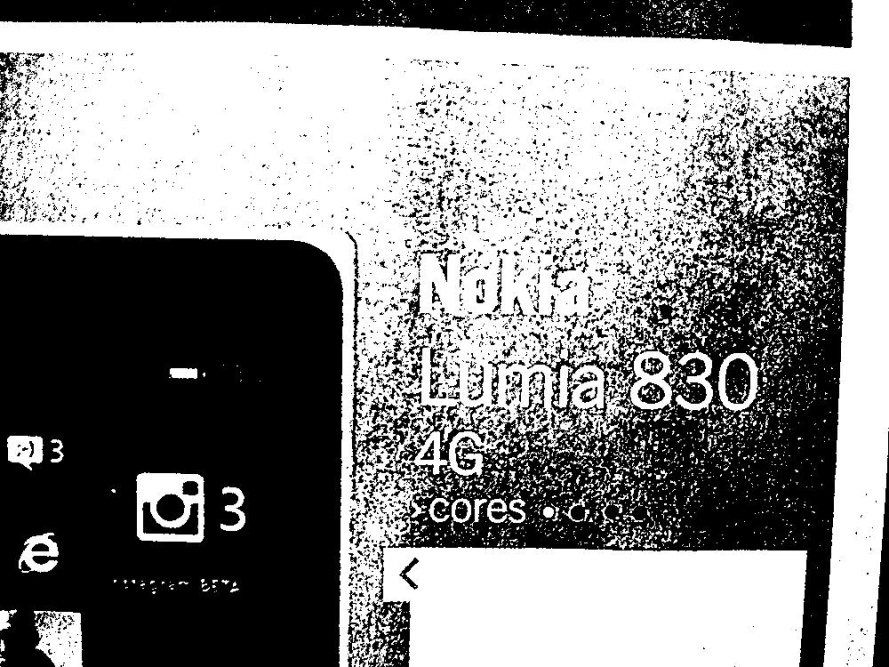
\includegraphics[width=0.4\textwidth]{fixed_threshold_01}
    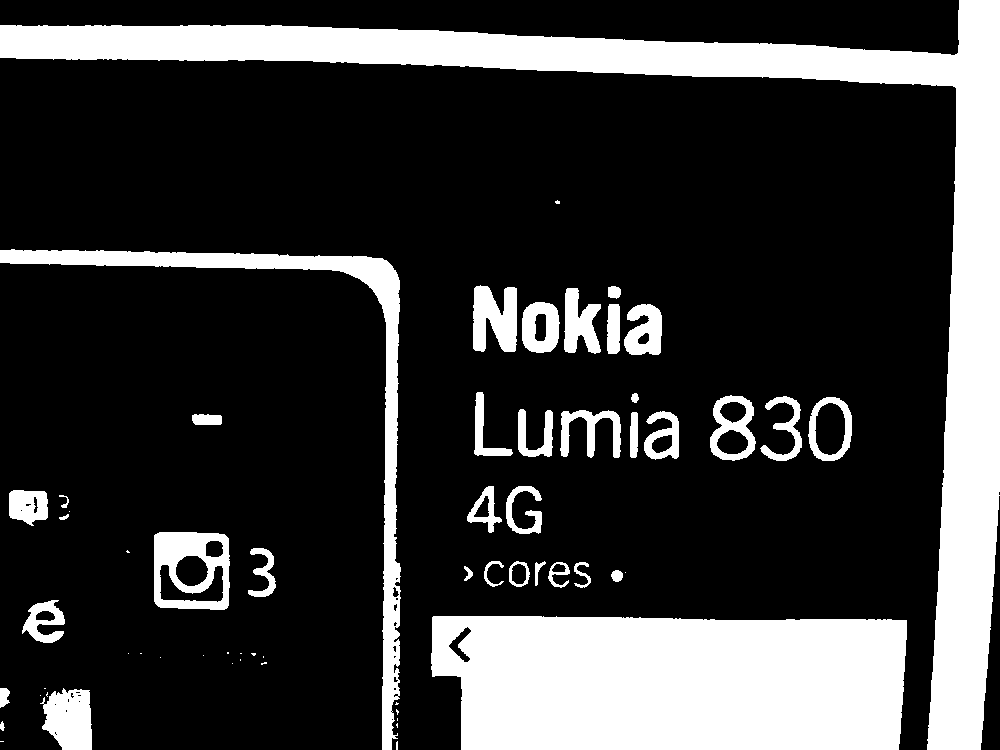
\includegraphics[width=0.4\textwidth]{fixed_threshold_02}
    \caption{Différents résultats à seuils fixes}
\end{figure}

Nous avons donc opté pour l'option du seuil automatique. Encore une fois il y a
de nombreux algorithmes pour implémenter une telle fonctionnalité, celui retenu
est la \textbf{méthode d'Otsu}. L'idée derrière cet algorithme est de construire
un histogramme pour analyser la distribution des intensités de gris de l'image,
puis de calculer un seuil optimal distinguant le premier plan et l'arrière-plan.

\begin{figure}[H]
    \centering
    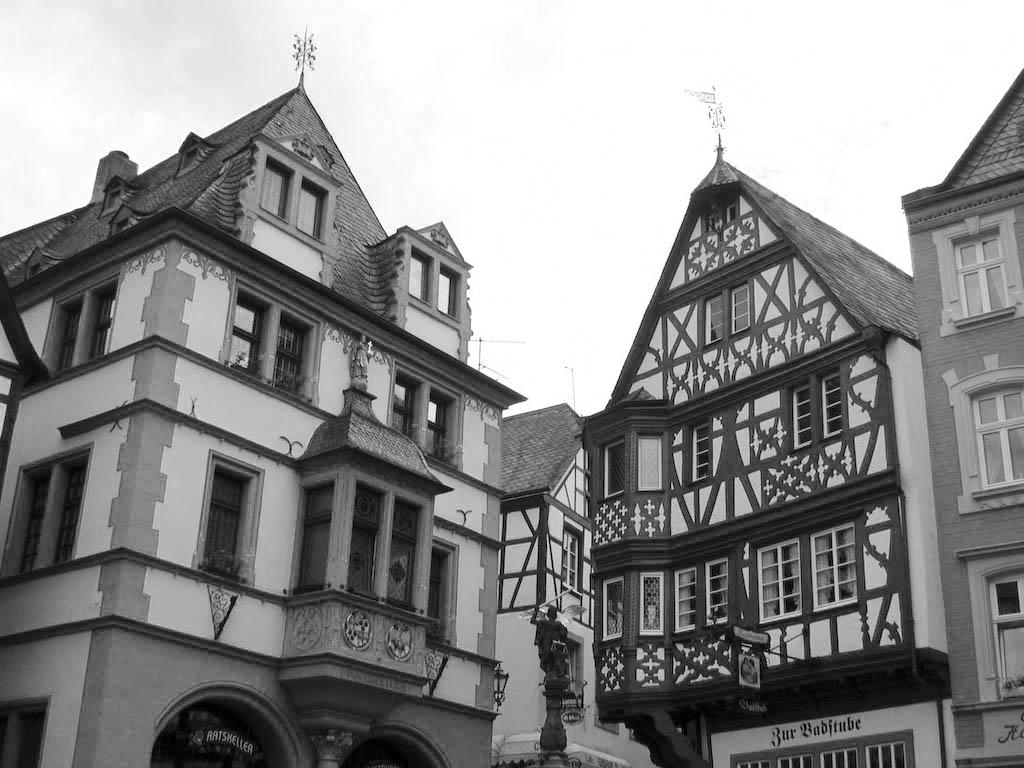
\includegraphics[width=0.45\textwidth]{houses}
    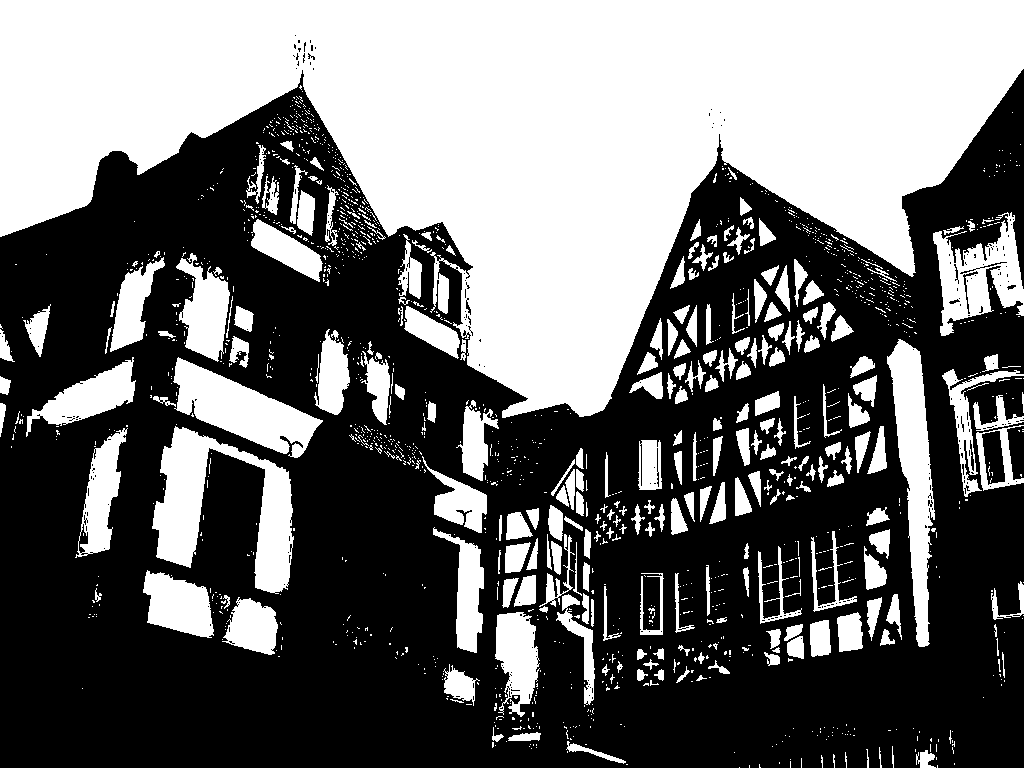
\includegraphics[width=0.45\textwidth]{houses_binarize}
    \caption{Binarisation à seuil automatique}
\end{figure}

\newpage

\section{Redressement de l'image}

Afin de faciliter la segmentation ainsi que le traitement de notre réseau de
neurones, il est nécessaire de redresser l'image. Pour trouver l'angle de
redressement optimal, la méthode employée teste différents angles et projette la
page afin de calculer un histogramme des pixels noirs.

\begin{figure}[H]
    \centering
    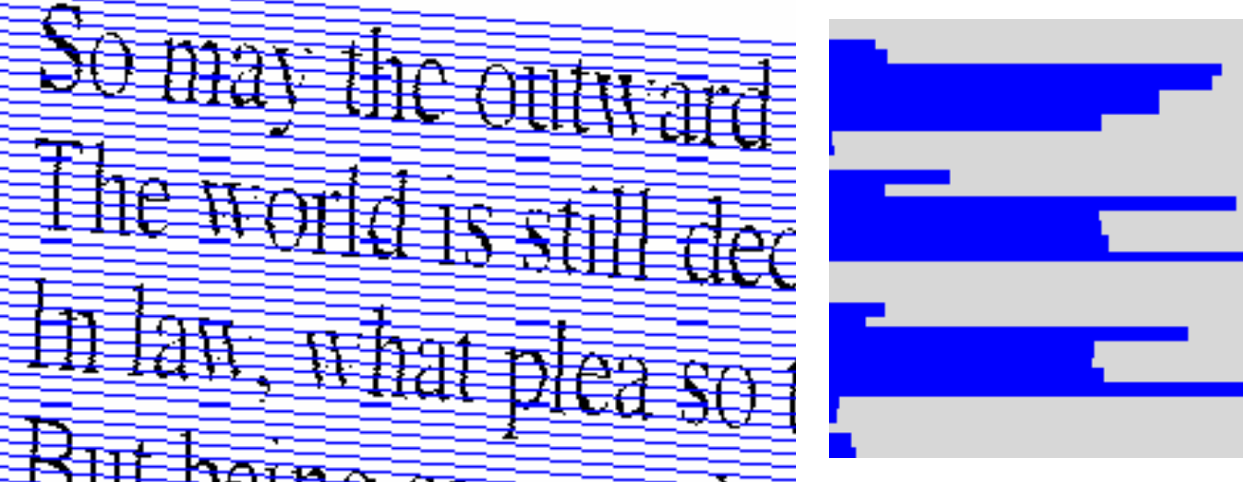
\includegraphics[width=0.7\textwidth]{skew_histogram01}
\end{figure}

\begin{figure}[H]
    \centering
    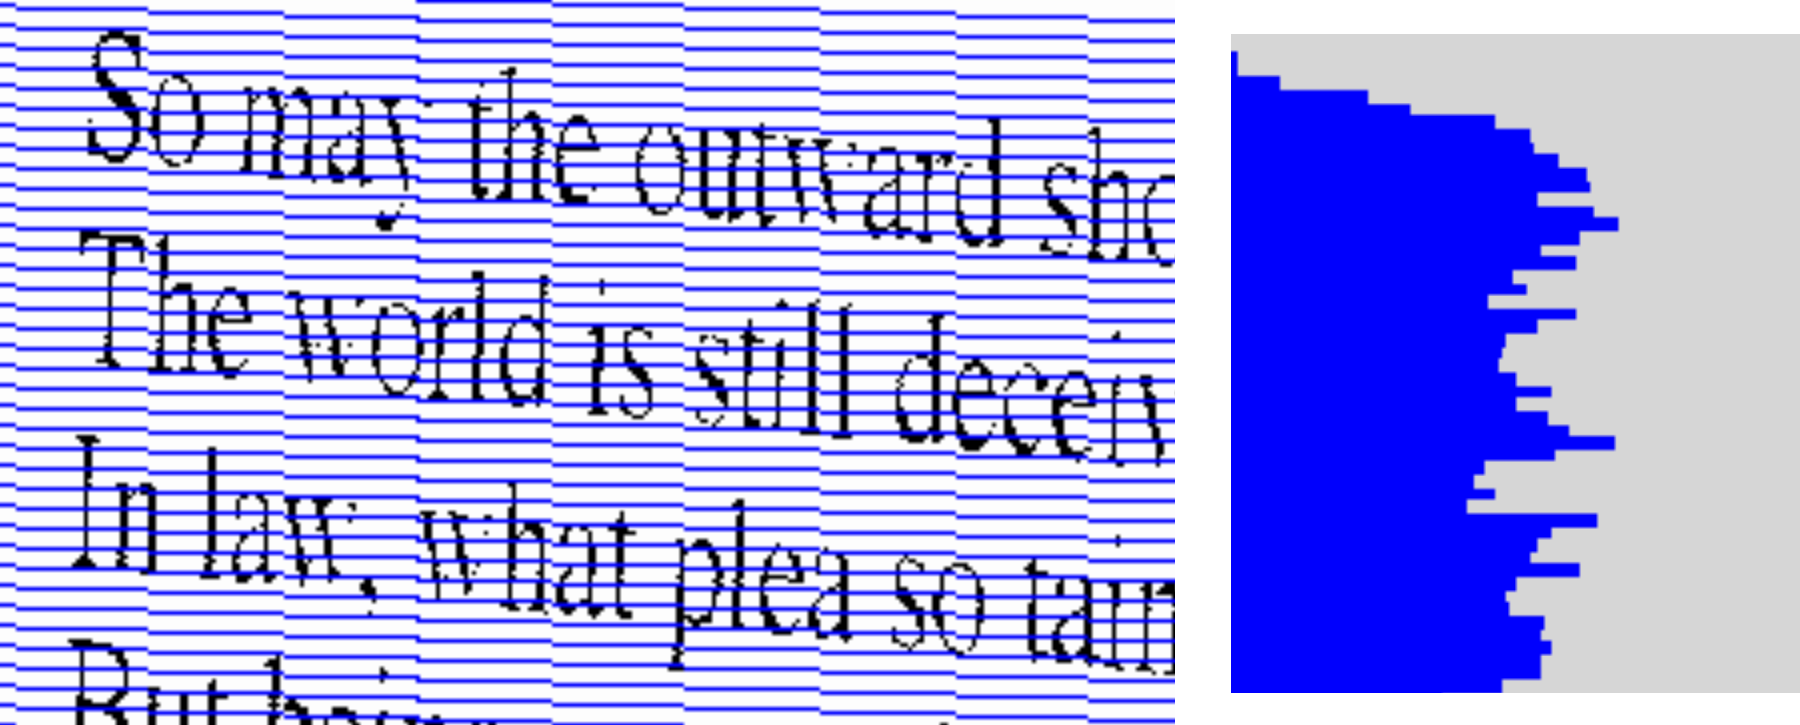
\includegraphics[width=0.7\textwidth]{skew_histogram02}
\end{figure}

Pour trouver un angle parallèle aux lignes du texte, il faut donc chercher à
maximiser la variance de l'histogramme calculé à chaque projection. La première
image
\footnote{\url{https://people.eecs.berkeley.edu/~fateman/kathey/skew.html}}
montre un cas où l'angle testé forme des lignes parallèles au texte,
l'histogramme obtenu a donc une variance élevée. Tandis que la deuxième image
utilise un angle résultant en des lignes obliques au texte, ce qui produit un
histogramme avec une faible variance.

\newpage

\section{Réduction du bruit}

Le dernier processus de pré-traitement de l'image de notre OCR est la réduction
du bruit. L'algorithme retenu est celui consistant à faire une moyenne des
couleurs des 8 pixels voisins pour éliminer les imperfections aléatoires de
l'image.

\begin{figure}[H]
    \centering
    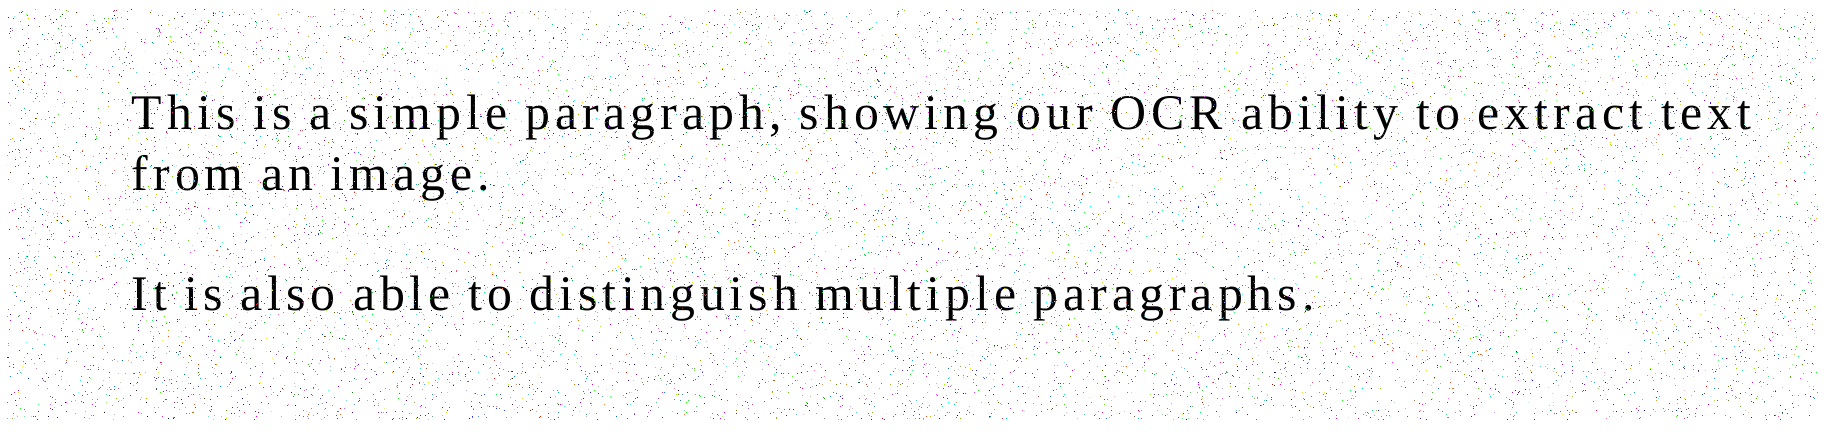
\includegraphics[width=0.8\textwidth]{image_noise}
    \caption{Image avec bruit aléatoire}
\end{figure}

\begin{figure}[H]
    \centering
    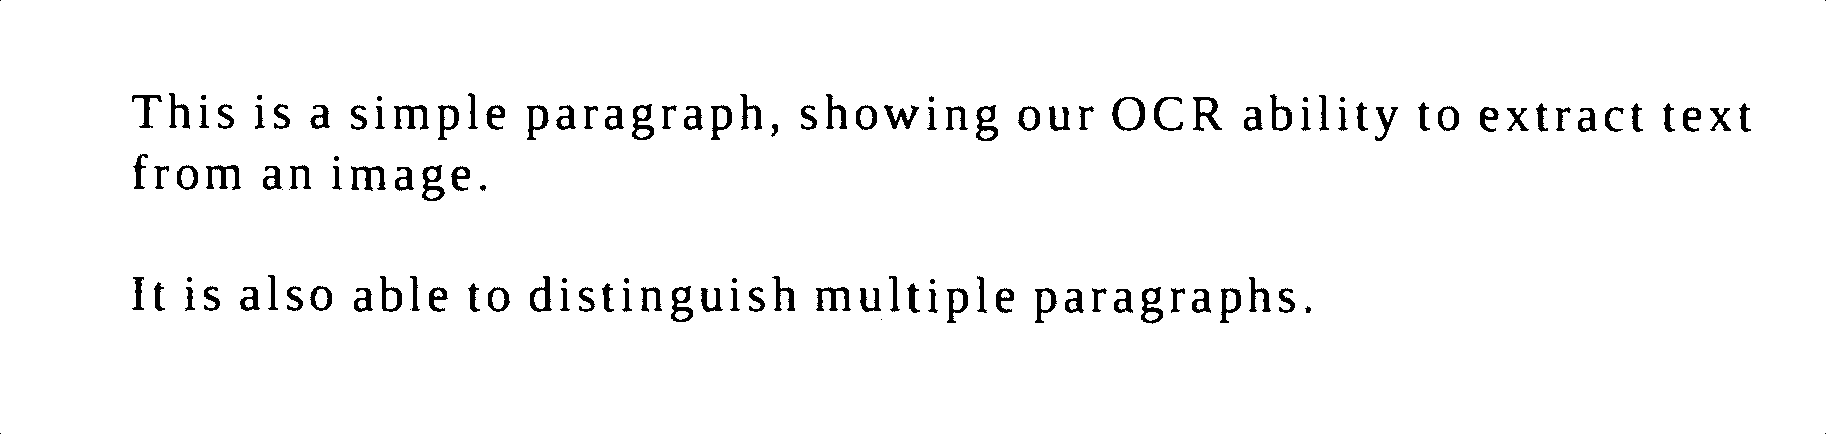
\includegraphics[width=0.8\textwidth]{image_noise_reduc}
    \caption{Résultat après réduction du bruit}
\end{figure}

D'autres méthodes de réduction ont été testées, comme celle du filtre médian,
mais les résultats étaient moins concluants pour notre application en
particulier (image déjà binarisée).
